\documentclass[tikz]{standalone}
\usetikzlibrary{shapes.geometric}    % trapezium
\usetikzlibrary{arrows}              % arrow tips
\usepackage{amsmath}
\usepackage{bm}                      % boldsymbol
\usepackage{makecell}                % makecell
\usetikzlibrary{matrix,calc}
\usepackage{color}
\usepackage{xcolor}
\definecolor{mygray}{HTML}{F0F0F0}

\begin{document}
    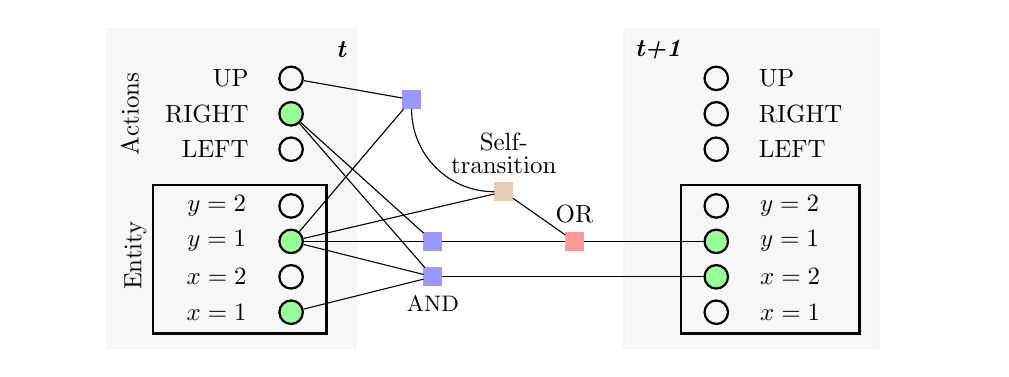
\begin{tikzpicture}[>=latex',thick, scale=0.9, every node/.style={scale=0.9}]]
      \coordinate (newcenter) at (0, 0);
      \coordinate (ydistance) at (0, 1);

      \node [name=c1] at ($(newcenter) + 1*(ydistance)$) {};
      \node [name=c4] at ($(newcenter) + 4.3*(ydistance)$) {};
      \node [name=UR] at ($(c4) + (2.12,0)$) {};
      \draw [fill=mygray, opacity=0.5, color=mygray] ($(c1) + (-2.6, -0.5)$) rectangle
      ($(UR) + (-1.2, 0.7)$);
      \node at ($(UR) + (-1.4, 0.4)$) {\textit{\textbf{t}}};

      \node [draw, circle, minimum size=5pt, name=c1, fill=green!40] at
      ($(newcenter) + 1*(ydistance)$) {};
      \node [align=right, name=UL] at ($(c1) + (-1.05,0)$) {$x=1$};
      \node [draw, circle, minimum size=5pt, name=c2] at
      ($(newcenter) + 1.5*(ydistance)$) {};
      \node [align=right] at ($(c2) + (-1.05,0)$) {$x=2$};
      \node [draw, circle, minimum size=5pt, name=c3, fill=green!40] at
      ($(newcenter) + 2*(ydistance)$) {};
      \node [align=right] at ($(c3) + (-1.05,0)$) {$y=1$};
      \node [draw, circle, minimum size=5pt, name=c4] at
      ($(newcenter) + 2.5*(ydistance)$) {};
      \node [name=UR, align=right] at ($(c4) + (-1.05,0)$) {$y=2$};

      \draw ($(UL) + (-0.9, -0.3)$) rectangle ($(c4) + (0.5, 0.3)$);

      \node [draw, circle, minimum size=5pt, name=c5] at
      ($(newcenter) + 3.3*(ydistance)$) {};
      \node [text width=3cm, align=right] at ($(c5) + (-2.10,0)$) {LEFT};
      \node [draw, circle, minimum size=5pt, name=c6, fill=green!40] at
      ($(newcenter) + 3.8*(ydistance)$) {};
      \node [text width=3cm, align=right] at ($(c6) + (-2.10,0)$) {RIGHT};
      \node [draw, circle, minimum size=5pt, name=c7] at
      ($(newcenter) + 4.3*(ydistance)$) {};
      \node [text width=3cm, align=right] at ($(c7) + (-2.10,0)$) {UP};

      \node [rotate=90] at ($(newcenter) + 1.8*(ydistance) + (-2.2, 0)$) {{Entity}};
      \node [rotate=90] at ($(newcenter) + 3.8*(ydistance) + (-2.27, 0)$) {{Actions}};

      \node [draw, rectangle, minimum size=5pt, fill=blue!40, color=blue!40, name=AND,
      label={[yshift=-0.75cm]\small{AND}}] at
      ($(newcenter) + 1.5*(ydistance) + (2, 0)$) {};


      \node [draw, rectangle, minimum size=5pt, fill=blue!40, color=blue!40, name=AND2,
      label={[yshift=0.00cm]}] at
      ($(newcenter) + 2*(ydistance) + (2, 0)$) {};


      \node [draw, rectangle, minimum size=5pt, fill=blue!40, color=blue!40, name=AND3,
      label={[yshift=0.00cm]}] at
      ($(newcenter) + 4*(ydistance) + (1.7, 0)$) {};


      \node [draw, rectangle, minimum size=5pt, fill=red!40, color=red!40, name=OR,
      label={[yshift=0.00cm]OR}] at ($(newcenter) + 2*(ydistance) + (4, 0)$) {};

      \node [draw, rectangle, minimum size=5pt, fill=red!40, color=brown!40, name=self,
      label={[align=center, yshift=0.00cm]Self-\\[-0.3em]transition}] at
      ($(newcenter) + 2.7*(ydistance) + (3, 0)$) {};

      \draw [-, thin] (c1) -- (AND);
      \draw [-, thin] (c3) -- (AND);
      \draw [-, thin] (c6) -- (AND);

      \draw [-, thin] (c3) -- (AND2);
      \draw [-, thin] (c6) -- (AND2);


      \node [name=c1] at ($(newcenter) + 1*(ydistance) + (6,0)$) {};
      \node [name=UR] at ($(newcenter) + 4.3*(ydistance) + (6, 0)$) {};
      \draw [fill=mygray, opacity=0.5, color=mygray] ($(c1) + (-1.3, -0.5)$) rectangle
      ($(UR) + (2.3, 0.7)$);
      \node at ($(UR) + (-0.8, 0.4)$) {{\textbf{\textit{t+1}}}};

      \node [draw, circle, minimum size=5pt, name=b1] at
      ($(newcenter) + 1*(ydistance) + (6, 0)$) {};
      \node [text width=3cm, name=UL] at ($(b1) + (2.12,0)$) {$x=1$};
      \node [draw, circle, minimum size=5pt, name=b2, fill=green!40] at
      ($(newcenter) + 1.5*(ydistance) + (6, 0)$) {};
      \node [text width=3cm, name=UL] at ($(b2) + (2.12,0)$) {$x=2$};
      \node [draw, circle, minimum size=5pt, name=b3, fill=green!40] at
      ($(newcenter) + 2.0*(ydistance) + (6, 0)$) {};
      \node [text width=3cm, name=UL] at ($(b3) + (2.12,0)$) {$y=1$};
      \node [draw, circle, minimum size=5pt, name=b4] at
      ($(newcenter) + 2.5*(ydistance) + (6, 0)$) {};
      \node [text width=3cm, name=UL] at ($(b4) + (2.12,0)$) {$y=2$};

      \node [draw, circle, minimum size=5pt, name=b5] at
      ($(newcenter) + 3.3*(ydistance) + (6, 0)$) {};
      \node [text width=3cm] at ($(b5) + (2.10,0)$) {LEFT};
      \node [draw, circle, minimum size=5pt, name=b6] at
      ($(newcenter) + 3.8*(ydistance) + (6, 0)$) {};
      \node [text width=3cm] at ($(b6) + (2.10,0)$) {RIGHT};
      \node [draw, circle, minimum size=5pt, name=b7] at
      ($(newcenter) + 4.3*(ydistance) + (6, 0)$) {};
      \node [text width=3cm] at ($(b7) + (2.10,0)$) {UP};

      \draw ($(b1) + (-0.5, -0.3)$) rectangle ($(UL) + (-0.1, 0.3)$);

      \draw [-, thin] (AND) -- (b2);
      \draw [-, thin] (AND2) -- (OR);
      \draw [-, thin] (self) -- (OR);
      \draw [-, thin] (c3) -- (self);
      \draw [-, thin] (OR) -- (b3);
      \draw [-, thin] (c7) -- (AND3);
      \draw [-, thin] (c3) -- (AND3);
      \draw [-, thin] (AND3) to [out=-90, in=-180] (self);
    \end{tikzpicture}
\end{document}
